%% LyX 1.1 created this file.  For more info, see http://www.lyx.org/.
%% Do not edit unless you really know what you are doing.
\documentclass[12pt,english]{article}
\usepackage[T1]{fontenc}
\usepackage[latin1]{inputenc}
\usepackage{babel}
\usepackage{graphics}

\makeatletter

%%%%%%%%%%%%%%%%%%%%%%%%%%%%%% LyX specific LaTeX commands.
\providecommand{\LyX}{L\kern-.1667em\lower.25em\hbox{Y}\kern-.125emX\@}

%%%%%%%%%%%%%%%%%%%%%%%%%%%%%% User specified LaTeX commands.
%%%%%
%%%%%
%%%%%
%% Welcome!
%% if you have any question about this
%% document, please get in touch with
%% Daniel Lemire at lemire@ondelette.com
%%
%% Of course, this file was generated
%% with LyX which means that the syntax
%% might be weird at times, but I've found
%% that LyX did an excellent job overall at
%% generating clean LaTeX syntax.
%% Why do I choose LyX? Because LyX
%% doesn't come with its own LaTeX engine.
%% LyX simply use whatever tex I have.
%% There is no "proprietary gizmos" going
%% on. Also, instead of waiting for support
%% from some folk in California, I can find
%% most of the answers I need on the web,
%% for free! Oh! And LyX is free too! 
%% Good old Open Source software!
%%
%% (Sorry for the propaganda!)
%% 
%% Thanks!
%% Enjoy!
%%
%% Sept. 8th 2001
%% Grand-Pr�, NS
%%
%%%%%%%%%%
%
% Notice that this document requires quite
% a bit of macros... 
% Sorry about that!
%%%%%%%%%%%%%%
%%
\usepackage{epsfig}
\usepackage{amsmath,amssymb}
\usepackage{pslatex}
\usepackage{color}
 
 \definecolor{veryblackblue}{rgb}{0.0,0.0,0.1}
 \usepackage[pdftex,urlcolor=webblackblue,colorlinks=true]{hyperref}
 \pdfinfo{
            /Title      (Introductory Calculus- Assignment 1 Solutions)
            /Author     (Daniel Lemire, Ph.D.)
            /Subject    (This is a set of solutions for sections 1.5, 1.6, 2.1, 2.2 and 2.3 in Stewart: calculus.)
            /Keywords   (exponentials, tangents, Stewart, Solutions, limits, Acadia)
          }


\topmargin  = 0pt
\headheight = 0pt
\headsep    = 0pt

\voffset    = 0in
\hoffset    = 0in
\textheight = 230mm
\textwidth  = 164mm

\evensidemargin = 0pt
\oddsidemargin  = 0pt

\pagestyle{empty}
\usepackage{float}

%% Background of blue palette
 \definecolor{webblackblue}{rgb}{0.0,0.0,0.2}
 \definecolor{webblue}{rgb}{0.0, 0.0, 0.6}

%% Background of red palette
 \definecolor{webblackred}{rgb}{0.2,0.0,0.0}
 \definecolor{webred}{rgb}{0.6,0.0,0.0}

%% Background of green palette
 \definecolor{webblackgreen}{rgb}{0.0,0.2,0.0}                                   
 \definecolor{webgreen}{rgb}{0.0,0.6,0.0} 

%% Background of magenta palette
 \definecolor{webblackmagenta}{rgb}{0.14,0.0,0.14}                                   
 \definecolor{webmagenta}{rgb}{0.42,0.0,0.42} 

%% Background of cyan palette
 \definecolor{webblackcyan}{rgb}{0.0,0.14,0.14}                                   
 \definecolor{webcyan}{rgb}{0.0,0.42,0.42} 

%% Background of yellow pallete
 \definecolor{webblackyellow}{rgb}{0.14,0.14,0.0}                                   
 \definecolor{webyellow}{rgb}{0.85,0.85,0.0} 

 \definecolor{webdarkgray}{rgb}{0.2,0.2,0.2}

 \definecolor{webgray}{rgb}{0.75,0.75,0.75}
 \definecolor{weborange}{rgb}{1.0, 0.6, 0.0}

\renewcommand\labelenumi{\textcolor{webdarkgray}{\arabic{enumi}.}}
\newcommand{\setenumi}[1]{#1.\setcounter{enumi}{#1}}
\usepackage{dsfont}
%%
%% You might need this next line... I don't for
%% some reason... defined somewhere?
%%
%% \newcommand{\setenumi}[1]{#1.\setcounter{enumi}{#1}}
%%
%% Document should begin NOW!
%%%%%%%%%%%%%%%%%%%%%%%
%%%%%%%%%%%%%%%%%%%%%%%

\makeatother
\begin{document}

\title{Acadia University \\
\href{http://ace.acadiau.ca/math/}{Department of Mathematics and Statistics}\\
 \vspace*{3mm} \textbf{INTRODUCTORY CALCULUS 1}\\
 (MATH 1013) \\
 \vspace*{3mm} ASSIGNMENT 1 Solutions}


\author{\href{http://ondelette.com/acadia/}{Daniel Lemire}, Ph.D.}

\maketitle
\tableofcontents{}

\setcounter{section}{1}


\section{\texorpdfstring{\textcolor{webblackblue}{Limits and Derivatives}}{Limits and Derivatives}}


\subsection{\texorpdfstring{\textcolor{webblue}{The Tangent and Velocity Problems}}{The Tangent and Velocity Problems}}

\begin{enumerate}
\item [\setenumi{2}]It is always useful to begin by plotting the points
we are given. You can do it very easily using Maple%
\footnote{Many different plotting tools can be used including Mathematica, gnuplot,
Matlab, Mathcad, EasyCalc (for Palm Pilot or Visor users). While you'll
learn to use Maple in this course, you can use any tool that suits
your needs. Some of them are free (gnuplot and EasyCalc for example).
} (see Fig. \ref{graphheart}).
\begin{figure}
[h]

{\centering \includegraphics{question2_1_2} \par}


\caption{\label{graphheart}Heartbeats vs minutes}
\end{figure}
 

\begin{enumerate}
\item We want to compute the slope of the secant line passing through \( \left( 36,2530\right)  \)
and \( \left( 42,2948\right)  \). Recall that the slope of the line
passing through \( \left( x_{1},y_{1}\right)  \) and \( \left( x_{1},y_{1}\right)  \)
is given my \[
m=\frac{y_{1}-y_{2}}{x_{1}-x_{2}}.\]
In the present case, we therefore have \[
m=\frac{2530-2948}{36-42}\cong 69.7.\]

\item We have to compute the slope of the secant line passing through \( \left( 38,2661\right)  \)
and \( \left( 42,2948\right)  \) which is\[
m=\frac{2661-2948}{38-42}=71.75.\]

\item We have to compute the slope of the secant line passing through \( \left( 40,2806\right)  \)
and \( \left( 42,2948\right)  \) which is\[
m=\frac{2806-2948}{40-42}=71.\]

\item We have to compute the slope of the secant line passing through \( \left( 42,2948\right)  \)
and \( \left( 44,3080\right)  \) which is\[
m=\frac{2948-3080}{42-44}=66.\]
 If we want to approximate the slope of the tangent line at \( 42 \),
we can look at the two closest secant lines (c and d) and expect the
slope of the tangent line to be somewhere between \( 66 \) and \( 71 \).
We can use the average of the two values \( \frac{66+71}{2}\cong 68.5 \)
as a good estimation for the heart rate in beats per minute at time
\( t=72 \).
\end{enumerate}
\item [\setenumi{4}]

\begin{enumerate}
\item We have have to compute the slope of the line passing through \( \left( 2,\ln 2\right)  \)
and \( \left( x,\ln x\right)  \) for some values of \( x \). The
general formula for the slope is going to be\[
m=\frac{\ln 2-\ln x}{2-x}.\]
Note that while the question in Steward require 6 decimal places values
for the slope, we give only 3 decimal places below.

\begin{enumerate}
\item For \( x=1.5 \), we have\[
m=\frac{\ln 2-\ln 1.5}{2-1.5}\cong 0.575.\]

\item For \( x=0.9, \) we have\[
m=\frac{\ln 2-\ln 0.9}{2-0.9}\cong 0.726.\]

\item For \( x=1.99, \) we have\[
m=\frac{\ln 2-\ln 1.99}{2-1.99}\cong 0.501.\]

\item For \( x=1.999, \) we have\[
m=\frac{\ln 2-\ln 1.999}{2-1.999}\cong 0.5.\]

\item For \( x=2.5, \) we have\[
m=\frac{\ln 2-\ln 2.5}{2-2.5}\cong 0.446.\]

\item For \( x=2.1, \) we have\[
m=\frac{\ln 2-\ln 2.1}{2-2.1}\cong 0.488.\]

\item For \( x=2.01, \) we have\[
m=\frac{\ln 2-\ln 2.01}{2-2.01}\cong 0.499.\]

\item For \( x=2.001, \) we have\[
m=\frac{\ln 2-\ln 1.5}{2-1.5}\cong 0.5.\]

\end{enumerate}
\item To guess the value of the slope, we look at the secant lines we get
with \( x=1.999 \) and \( x=2.001 \), they both have a slope of
\( \approx 0.5 \) and therefore, \( m=0.5 \) is our best guess.
\item The tangent line will have a slope of \( 0.5 \) and therefore, its
equation is going to be\begin{equation}
\label{linehalf}
y=0.5x+b
\end{equation}
 and it remains to solve for \( b \). We know that the tangent line
must pass through \( \left( 2,\ln 2\right)  \) and so we substitute
these values in equation \ref{linehalf}. Solving for \( b \), we
get\[
b=\ln 2-0.5\times 2=\ln 2-1\cong -0.306.\]
We therefore have the equation \[
y=0.5x-\ln 2+1.\]

\item Before sketching, we may compute the actual equations for the second
lines. Choosing \( x=1.5 \) and \( x=2.5 \) from part a, we have
to solve for \( b \) in the following equations\[
0.575\times 2+b=\ln 2\]
and\[
0.446\times 2+b=\ln 2.\]
It is, of course, very easy. We get \( b\cong -0.457 \) and \( b\cong -0.198 \)
respectively. For sketch, see Fig. \ref{graphtangents}
\begin{figure}
[h]

{\centering \includegraphics{question2_1_4} \par}


\caption{\label{graphtangents}The tangent line and two secant lines at \protect\( x=2\protect \)
for the curve \protect\( y=\ln x\protect \).}
\end{figure}
 
\end{enumerate}
\item [\setenumi{6}]We plot the height as a function in time (see Fig. \ref{graphgalileo}).
\begin{figure}
[h]

{\centering \includegraphics{question2_1_6} \par}


\caption{\label{graphgalileo}\protect\( h=58t-0.83t^{2}\protect \)}
\end{figure}
 

\begin{enumerate}
\item Computing the average velocity is very similar to computing the slope
of a secant line as we shall see.

\begin{enumerate}
\item The average velocity is given by\[
\frac{\left( 58\times 1-0.83\times 1^{2}\right) -\left( 58\times 2-0.83\times 2^{2}\right) }{1-2}=55.51.\]

\item The average velocity is given by\[
\frac{\left( 58\times 1-0.83\times 1^{2}\right) -\left( 58\times 1.5-0.83\times 1.5^{2}\right) }{1-1.5}=55.925.\]

\item The average velocity is given by\[
\frac{\left( 58\times 1-0.83\times 1^{2}\right) -\left( 58\times 1.1-0.83\times 1.1^{2}\right) }{1-1.1}=56.257.\]

\item The average velocity is given by\[
\frac{\left( 58\times 1-0.83\times 1^{2}\right) -\left( 58\times 2-0.83\times 1.01^{2}\right) }{1-1.01}=56.3317.\]

\item The average velocity is given by\[
\frac{\left( 58\times 1-0.83\times 1^{2}\right) -\left( 58\times 1.001-0.83\times 1.001^{2}\right) }{1-1.001}=56.33917.\]

\end{enumerate}
\item We can estimate from the previous results that the velocity at \( t=1 \)
is going to be \( 56.34 \).
\end{enumerate}
\end{enumerate}

\subsection{\texorpdfstring{\textcolor{webblue}{The Limit of a Function}}{The Limit of a Function}}

\begin{enumerate}
\item [\setenumi{4}]

\begin{enumerate}
\item We have a continuous function at \( x=0 \) and the limit from both
sides will tend to \( 3 \).
\item If we come from the left, the limit will tend to \( 4 \) even though
it might not agree with the limit from the right or the value of the
function at \( x=3 \).
\item This time, the limit tends to \( 2 \) even though it doesn't agree
with the limit from the left and the value of the function at \( x=3 \).
\item From our previous comments, the limits from the left and from the
right don't agree so that the limit doesn't exist (see \cite[section 2.2, equation 3]{Steward})
\item Even though, it might seem strange, the value of \( f(3) \) is simply
\( 3 \).
\end{enumerate}
\item [\setenumi{6}]We sketch the graph of the function \( f \) using our
favorite software package (in this case, we are using gnuplot, see
Fig. \ref{graphdiscontinuous}). For the graph, it is clear that \( \lim _{x\rightarrow -1}f(x) \)
and \( \lim _{x\rightarrow 1}f(x) \) do not exist. Other than than,
all limits will exist so that the set we are looking for is \( \mathds {R}-\{-1,1\} \).
\begin{figure}
[h]

{\centering 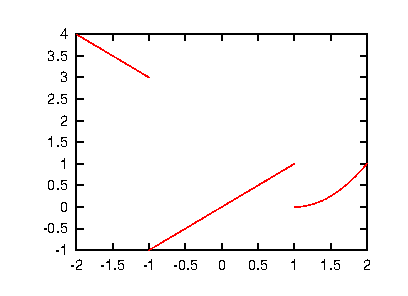
\includegraphics{question2_2_6} \par}


\caption{\label{graphdiscontinuous}The discontinuous function \protect\( f(x)\protect \).}
\end{figure}
 
\item [\setenumi{16}]

\begin{enumerate}
\item We plot\( \frac{6^{x}-2^{x}}{x} \) near \( x=0 \) using our favorite
plotting software (see Fig. \ref{graphexp62}). Clearly we have that
the limit must be closed to \( 1.10 \).
\begin{figure}
[h]

{\centering \includegraphics{question2_2_16} \par}


\caption{\label{graphexp62}The function \protect\( \frac{6^{x}-2^{x}}{x}\protect \)
near \protect\( x=0\protect \).}
\end{figure}

\item Evaluating \( \frac{6^{x}-2^{x}}{x} \) at \( x=0.0001 \), we get
\( \approx 1.098 \) and at \( x=-0.0001 \), we get \( \approx 1.098 \)
and therefore \( 1.10 \) is clearly a good choice.
\end{enumerate}
\item [\setenumi{18}]

\begin{enumerate}
\item We use our calculator to get\[
\frac{\tan 1-1}{1^{3}}\cong 0.5574,\]
\[
\frac{\tan 0.5-0.5}{0.5^{3}}\cong 0.3704,\]
\[
\frac{\tan 0.1-0.1}{0.1^{3}}\cong 0.3347,\]
\[
\frac{\tan 0.05-0.05}{0.05^{3}}\cong 0.3337,\]
\[
\frac{\tan 0.01-0.01}{0.01^{3}}\cong 0.3333,\]
\[
\frac{\tan 0.005-0.005}{0.005^{3}}\cong 0.3333.\]

\item Since values tend to go to \( 1/3 \) when \( x \) goes down to \( 0 \),
we must assume that the limit will tend to \( 0 \).
\item Using a calculator, we get \( 0 \) for values around \( 1\times 10^{-8} \)%
\footnote{Smarter calculators may still print a non-zero value, but no matter
what, you'll eventually get small enough values for your calculator
to print \( 0 \). Just try smaller values for \( x \).
}. Looking closely at the problem, we see that \( \tan x-x \) has
value \( 0 \) on the calculator for \( x=1\times 10^{-8} \), whereas
\( x^{3}=1\times 10^{-24} \). Why do we get \( \tan x-x=0 \) instead
of \( \sim x^{3}/3\cong 3\times 10^{-25} \)? First of all, what is
\( \tan x \) when \( x=1\times 10^{-8} \)? Simply \( 1\times 10^{-8} \),
of course, which explain why we get \( \tan x-x=0 \) in the first
place! We might expect \( \tan x=1\times 10^{-8}+3\times 10^{-25} \)
instead... but wait! Can your calculator manage a number like \( 1\times 10^{-8}+3\times 10^{-25} \).
Of course not! For most calculator, \( 3\times 10^{-25} \) is just
too small with respect to \( 1\times 10^{-8} \) and it will just
be discarded. Therefore, we are still confident about the value of
our limit being \( 1/3 \) and that the zero values come from numerical
error.
\item We use our favorite plotting package... See Fig. \ref{graphlimittan}
and \ref{graphlimittanstress}. We can see on Fig. \ref{graphlimittanstress}
how the graphing tool has problems with values very close to \( 0 \)
since the curve doesn't seem to be as smooth as one would expect and
it eventually goes to \( 0 \). Notice that scientists often get around
these problems by changing the units they are using.
\begin{figure}
[h]

{\centering \includegraphics{question2_2_20a} \par}


\caption{\label{graphlimittan}The function \protect\( \frac{\tan x-x}{x^{3}}\protect \)
.}
\end{figure}

\begin{figure}
[h]

{\centering \includegraphics{question2_2_20b} \par}


\caption{\label{graphlimittanstress}The function \protect\( \frac{\tan x-x}{x^{3}}\protect \)
very near \protect\( x=0\protect \). Notice how we stress the floating
point lower limit of our graphing tool as \protect\( x\protect \)
tends to 0.}
\end{figure}

\end{enumerate}
\end{enumerate}

\subsection{\texorpdfstring{\textcolor{webblue}{Calculating Limits Using the Limit Laws}}{Calculating Limits Using the Limit Laws}}

\begin{enumerate}
\item [\setenumi{6}]We have that\begin{eqnarray}
\lim _{u\rightarrow -2}\sqrt{u^{4}+3u+6} & = & \sqrt{\lim _{u\rightarrow -2}u^{4}+3u+6}\label{deleteme} \\
 & = & \sqrt{\lim _{u\rightarrow -2}u^{4}+\lim _{u\rightarrow -2}3u+\lim _{u\rightarrow -2}6}\label{deleteme2} \\
 & = & \sqrt{\left( \lim _{u\rightarrow -2}u\right) ^{4}+3\lim _{u\rightarrow -2}u+\lim _{u\rightarrow -2}6}\label{deleteme3} \\
 & = & \sqrt{\left( -2\right) ^{4}+3\times -2+6}\label{deleteme4} \\
 & = & \sqrt{16}=4
\end{eqnarray}
by using respectively the Root Law (equation \ref{deleteme}), Law
1 (equation \ref{deleteme2}), the Power Law and Law 3 (equation \ref{deleteme3})
and Laws 7 and 8 (equation \ref{deleteme4}).
\item [\setenumi{8}]

\begin{enumerate}
\item It is not true when \( x=2 \) because the right hand side isn't defined
(division by 0).
\item The limit of a function at \( x=2 \) doesn't depend on the value
of the function at \( x=2 \) itself, but only on the values nearby.
Since the equality presented in question a is true everywhere but
at \( x=2 \), this new equation is correct.
\end{enumerate}
\item [\setenumi{10}]We have that \( \lim _{x\rightarrow -4}x^{2}+3x-4=0 \)
and therefore, we cannot use the quotient rule. Notice however that
\[
\frac{x^{2}+5x+4}{x^{2}+3x-4}=\frac{\left( x+4\right) \left( x+1\right) }{\left( x+4\right) \left( x-1\right) }\]
and so, for \( x\neq -4 \), we can consider\begin{equation}
\label{xmoinsxplus}
f(x)=\frac{\left( x+1\right) }{\left( x-1\right) }
\end{equation}
instead. Now, it is much easier because we can use the quotient rule.\begin{eqnarray*}
\lim _{x\rightarrow -4}\frac{\left( x+1\right) }{\left( x-1\right) } & = & \frac{\lim _{x\rightarrow -4}\left( x+1\right) }{\lim _{x\rightarrow -4}\left( x-1\right) }\\
 & = & \frac{\lim _{x\rightarrow -4}x+\lim _{x\rightarrow -4}1}{\lim _{x\rightarrow -4}x-\lim _{x\rightarrow -4}1}\\
 & = & \frac{-4+1}{-4-1}=\frac{3}{5}.
\end{eqnarray*}

\item [\setenumi{12}]We must first simplify the function for \( x\neq 1 \),\[
\frac{x^{3}-1}{x^{2}-1}=\frac{\left( x-1\right) \left( x^{2}+x+1\right) }{\left( x-1\right) \left( x+1\right) }=\frac{x^{2}+x+1}{x+1}\]
and now, we can use the Quotient Law,\begin{eqnarray*}
\lim _{x\rightarrow 1}\frac{x^{3}-1}{x^{2}-1} & = & \lim _{x\rightarrow 1}\frac{x^{2}+x+1}{x+1}\\
 & = & \frac{\lim _{x\rightarrow 1}x^{2}+x+1}{\lim _{x\rightarrow 1}x+1}\\
 & = & \frac{3}{2}.
\end{eqnarray*}

\item [\setenumi{26}]We use the Squeeze Theorem (see \cite[Theorem 3 in section 2.3]{Steward}).
We have that\[
\lim _{x\rightarrow 1}3x\leq \lim _{x\rightarrow 1}f(x)\leq \lim _{x\rightarrow 1}x^{3}+2\]
and therefore\[
3\leq \lim _{x\rightarrow 1}f(x)\leq 3\]
 which implies \[
\lim _{x\rightarrow 1}f(x)=3.\]

\item [\setenumi{30}]On the one hand, we have \[
\lim _{x\rightarrow 2^{-}}\frac{\left| x-2\right| }{x-2}=\lim _{x\rightarrow 2^{-}}\frac{2-x}{x-2}=-1\]
and on the other, we have \[
\lim _{x\rightarrow 2^{+}}\frac{\left| x-2\right| }{x-2}=\lim _{x\rightarrow 2^{+}}\frac{x-2}{x-2}=1.\]
Clearly, the limit doesn't exist!
\end{enumerate}
\begin{thebibliography}{Stewart}
\bibitem[Stewart]{Steward}James Stewart, \textit{Calculus: Concepts and Contexts} (Second Edition),
Brooks/Cole, 2001.\end{thebibliography}

\end{document}
